\documentclass{article}
\usepackage{graphicx}
\usepackage{titling}
\usepackage[a4paper, total={7in, 8in}]{geometry}

\setlength{\droptitle}{-10em}

\title{WebApps Project - Music Collaboration}
\author{Ashley Hemingway, Charchris Sloan, \\ David Liskevich, Edwin Kamulegeya \\ Group 9 (g1327109)}
\date{\today}

\begin{document}
\maketitle

\section{Introduction}
\subsection{Overview}
During discussions to find a suitable web app, it was discovered that a few members of the group had problems when trying to develop music. The main reason for this problem was that there were only skilled in certain aspects of the music development process, not possessing the skills for other parts and thus requiring help from people with different or more developed skill sets. This is where the idea for our web app came from, allowing people from all over the world to help each other to make music together. This lead to the overall idea of allowing album designers, lyricists and musicians to come together to actually make a musical product.\\
We also wanted to make a unique app, which either was a brand new original idea or one which improved on limited existing apps. With further research into our proposed solution it was discovered that a similar app already existed, although it was below our expectations and lacked a clean user friendly interface with good functionality. This is why we decided to continue with our original app idea, but to make it much better than the existing app.\\
The solution for this problem will be discussed in much further depth in later sections.
\subsection{Requirements}
Considering our web app deals with music collaboration, below are the required functionality of the web app.
\begin{itemize}
  \item Home Page which is simple and straight to the point, allowing for easy access to sign up or to login in to an already existing account.
  \item Profile pages which allow for users to keep track of their own songs and album artwork created via the web app. It will allow for easy uploading and downloading of files while giving the ability for the user to change the information about themselves.
  \item The ability to create a project, specifying the type of help required and the genre of the music associated with the project.
  \item Users must be invited by the project owner to join and collaborate within a specific project.
  \item Within a project, it will allow members of the project to add new music and album art to be upvoted/downvoted by members.
  \item A top featured page showing the top rated music and best collaborators.
  \item The ability to search via users, projects, genres and music files.
  \item Group chat between all members of each project to discuss the way the project is developing.
  \item Ability to rate the help and contribution of users.
\end{itemize}
\subsection{Targets}

\begin{itemize}
  \item We would like to add a workflow, so if remixes are made, they can be kept track of.
  \item Contests is another feature we would like to add. It would allow smaller artists to gain publicity, and also garner more interest in the website, as smaller musicians have a better chance. This could only really be done when a large fanbase was established.
  \item Add comments to certain parts of the track, this would be akin to soundclouds comments.
  \item If we had more time and the proper resources, we certainly would like to add a support sections for our users, so that they hone their skills. One aspect would be tutorials sections which would actively help our users. Another would be a problem page, where if users are having trouble with software or instrutments they can ask for help from users. 
  \item Licences are crucial to protecting musical rights. We are going to add the option for the use to choose their own license, e.g. make it public and waive all rights.
  \item Add a podcast/ soundcloud account to showcase all the highly rated music.
\end{itemize}

\subsection{Alternative Apps}
During our discussions, as a group we also came up with other numerous ideas which shall be mentioned. \\
We firstly discussed the idea of a lending network app which would allow people to keep track of items which they have leant to other people, while being a place to ask to borrow items from other people and be helpful and lend things to friends. We found none of us were passionate about this idea, as none of us found lending things to be much of a problem. \\
Secondly, we thought of making a game which would allow interaction for multiple users via handheld devices, but the overall game would be played on a computer. Basically the handheld device would act as your own personal game management screen while the computer would keep track of the overall game. We liked the initial idea, however, we thought that the overall concept would be too hard to implement due to our time frame and the lack of experience in the team. \\
Finally, we wanted to build a web app which would allow people to basically build their own website containing of their customised RSS feeds. We liked this proposed idea as it would allow us to extend it with features when needed, although we diverged away from this idea in the end as we though it lacked a full user interaction experience as required, while also being challenging enough to implement.
\section{Project Management}
\subsection{Group Structure}
Obviously, it would have been ideal for every member of the group to sample every part of the development stage, whether that was the back-end or front-end implementation. In practice, we decided to split the group up into the front-end and back-end sections, mainly because none of us had experience in this type of development, so we would have to learn everything from the start. Splitting the group up meant we could focus on one section and become an expert in this section, allowing for a better end product.\\
The back-end was mainly handled by Ashley Hemingway, who designed the database structure, wrote the database interaction code in PHP and implemented all the handling the constant data being pulled with Ajax and JavaScript.\\
The front-end was handled by the other group members (Charchris Sloan, David Liskevich \& Edwin Kamulegeya). Their main job was to design the user interface and carry out the implementation, using multiple languages like HTML, CSS and JavaScript/jQuery.\\
The group was split up like this, as we decided that the web app design and user interaction should be the main feature, allowing the web app to be easy and intuitive to use. This meant that 3 people focussed on this area. The main problem with this decision was the obvious disparity between the front-end and back-end development, meaning that we somehow had to bring these differences back together for the final product. This was done via constant interaction between the group members, meaning that the front-end and back-end was could be constantly be linked together during the development stage once certain sections were completed. For example, once the homepage design had been implemented by Edwin, David and Charchris, this allowed the homepage to be passed to Ashley in order to complete the form validation and the interaction with the database.
\subsection{Implementation Languages}
Below are the choices of coding languages we chose to implement out web app in. Although there are many to pick from, we thought that the combination of all of these, combined with our knowledge of web app design, would give us the best chance of producing a highly polished and functional website.
\subsubsection{HTML/CSS}
HTML and CSS were an obvious choice. Their popularity is down to the fact that they are the best basis to design a website on and require no specific software or hardware other than a compatible web browser. HTML is offers all of the functionality required simply and with no limitation on use, and combined with CSS to easily to change the look of the website, it is the perfect choice. HTML also neatly interacts with JavaScript/jQuery and PHP which is a massive advantage. Furthermore, the newly updated HTML5 offers even more functionally like 'drag and drop' and embedded audio which are both requirements of the web app. Both languages are structured very easily and are extendable easily.
\subsubsection{Bootstrap}
Bootstrap was chosen because it basically allows us to development a great looking website from scratch. As a group we were wary of using a website template as it wouldn't give us the best learning experience, so we decided to use the Bootstrap components when required. This allows us to keep a constant design throughout the whole of the website while making the trivial component coding not necessary, meaning we can focus more on the user experience and functionality.
\subsubsection{JavaScript/jQuery}
JavaScript enables us to add better usability to the website while also keeping things simple. It is widely supported and offers a vast array of frameworks to help us, most noticeably jQuery. It will become very useful when implementing such features like form validation and easing effects to provide the website with an enhanced user experience. Furthermore, JavaScript is a requirement when using Ajax, which we will discuss later.
\subsubsection{PHP}
Although there are many options to code the back-end in like Node, Django, Ruby, Python and Java we decided to choose PHP. The main reason behind this was that PHP is widely used and it is therefore very stable, with many tutorials and supporting libraries. Since none of us have any experience with developing the back-end of a web app, we decided that this would give us the best learning experience. It also offers and easy to use interaction with the PostgreSQL database and means we can push and pull from the database when required via the use of Ajax. It also had great functionality when it came to data encryption and JSON (JavaScript Object Notation) which benefitted us when transferring data between the server and client.
\subsubsection{Ajax}
Ajax became an important part of the app as it allowed us to pull and store data from the database, without the need for a page refresh. As a major part of our app is to do with user experience this became very useful. Since we were implementing our app in JavaScript/jQuery, using Ajax was an obvious choice as the major functionality is already included in those frameworks, while the server side data handling was relatively easy as well. Ajax became useful for features like the user chat and the constant updating of the top featured music. There aren't many alternatives to Ajax available, and since our app doesn't require an immediate update (i.e. it can wait 0.5 seconds to get the latest data) it is the best technology at our disposal.
\subsection{Design Processes}
\subsection{Back-up Systems}
Due to the fact that we are using the provided Virtual Machine to run our server and PostgreSQL database on, backing up the data is imperative as the VM isn't backed up automatically. In order to back-up the web page data/scripts (e.g. PHP scripts, css, html, JavaScript), we have been using GitHub. This was a great platform to use, as it allowed is to back-up our work, roll back to a previous stage of the design process and to easily share our work throughout the whole group on different devices. The choice to use GitHub over GitLab didn't really cross our mind as they both provide the functionality of git, while been both easily accessible. \\
\newline
As we were using a large database storing multiple values for all aspects of the app, it was also important that the database didn't become corrupt or lost. In order to stop this from happening, we implemented an auto-back-up feature on the VM so the database would be automatically back-up every day, allowing us to restore to previous points when required. This became very useful when playing around with data inserts, as on occasions this didn't work as expected.

\section{Actual App}
\subsection{Program Description}
Our application is a network which allows users to collaborate and share their musical projects, as well as seek expertise from people with more developed skills.One can display a project and split it up into sections however one likes, be it by instrument, chronological order or by role in the composition. It allows Followers of projects to vote(star) files uploaded in each section of a project to allow the owner/s of a project to have widespread feedback on what direction their project should take.
\subsection{Implementation}
\subsubsection{Homepage}
Upon loading the homepage, we decided that this experience should be minimal in what it is trying to get across. We wanted to explain quickly and formally what we want to accomplish and what the site offers. It needed to get encourage signing up as fast as possible, so we decided to make this the main focus of the homepage. \\

Two sections ease into the page, one section pushing towards making an account and the second section describing the website. We thought that this was more appropriate as opposed to delegaing these features to their own individual pages. \\ 

Lastly, we made use of a unique navigation bar on the homepage where a registered user will login to their profile page. It is unique in the fact that when a user logs in, there is a persistent navigation bar that used used between different pages and is used in an interconnected fashion.

\subsubsection{Profile Page}
The remaining pages focus on when the user has logged into the site. It is at this point where we make use of our consistent navigation bar that contains a search bar, button to create a new project, the name of the site and a dropdown box labelled as the username. The dropdown box consists of buttons to direct the user to other parts of the site and can log the user out of their session. We felt that this is what the user needed these options at all times withoiut having to bury deep into the interface to access sections of the site. Creating a new page was dedicated to a pop-out modal so that the user doesn't need to unneccisarily leave the page. \\

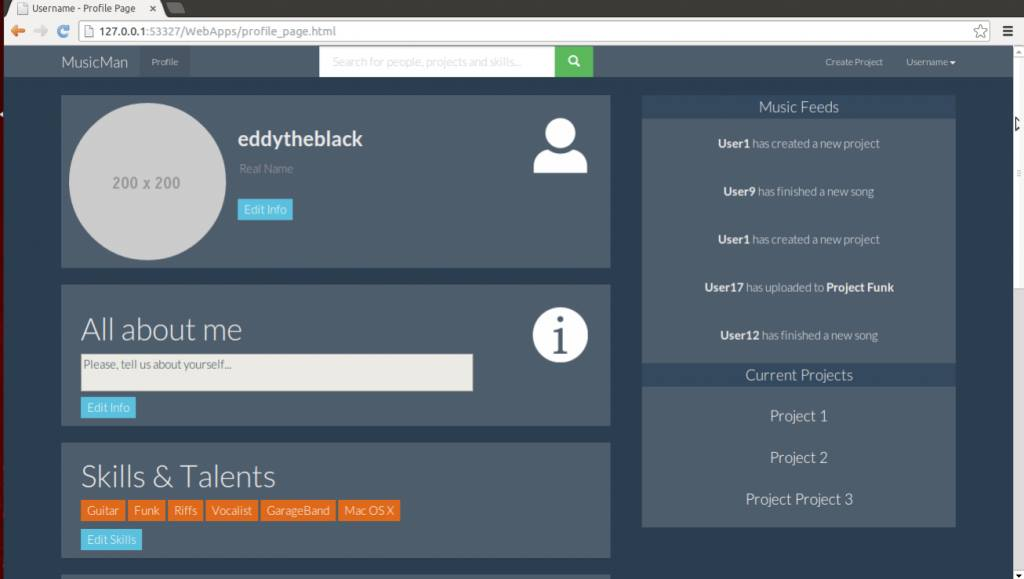
\includegraphics[width=180mm]{3.jpg}

The profile page has been split into six important sections. These being the user area, the descption section, skills \& talents, sounds, album portfolio and a side bar newsfeed. \\ 

The user area simply displays a neat profile picture of the user, their name and username in a clear manner. The profile picture can be changed at anytime and be loaded into the database. The description area is where the user can express themselves as creativly as they desire. They can talk about themselves, their experience and what drives their passion artistically.\\

The skills and talents section highlights what they can bring to a project they are looking for. These are expressed as tags on the website, where each tag can act as a quick search if you are viewing somebody else's profile. Skills can be removed by simply closing a them as you would close a standard window (e.g browser window). When a search is being made for certain skills across the database, matching profiles are determined by the Skills \& Talents section. This would ideally extend with an endorsement system.\\ 

The sound section is where a user can upload their personal collection of sounds for others to listen to. It is simply a pleasant way to share sounds and mixes with a community of users. The same principle goes with the album portfolio. A user can showcase the album artwork of their latest projects, or they can show what they have drawn themselves or created in some other software. \\

Lastly, we have a sidebar that is persistent across all pages on the website. It is a part of the site that contains a feed system on the site and a list of projects a user is currently working on. The feed system is a bit more sophisticated in that it contains constant updates on different users and what they are up to. These include whether a user you are following or interested in has created a new project, finished a song or have uploaded to a project they'r 


\subsubsection{Project Page}
The constant navigation bar continues through to the project page, giving the site a consistent feel and use throughout. \\

There is a section at the top called the project header with contains album art for the project and all necessary information about the project, to easily convey the idea and the progress of the project to any users which come across it.\\ 

Below that there is a variable number of separate sections for each section of the project, as split by the user. We chose this layout as it allows the page to dynamically grow for larger projects without having to change the layout of the entire page, more sections are simply added at the bottom. Each section has 3 sections, an easy to use, custom designed interface for the audio player, a list of all files submitted and a description for the file, to show each section being separate at this stage from another \\ 

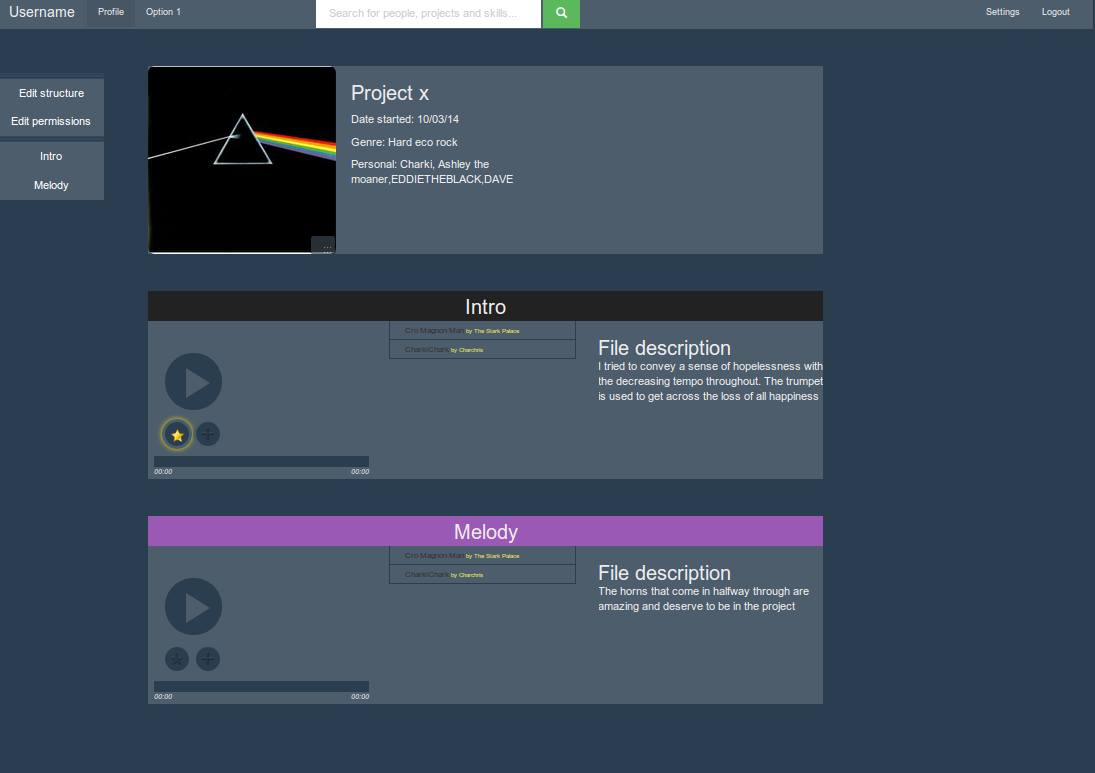
\includegraphics[width=180mm]{2.jpg}

Since the number of sections has no limit, the page could grow to be cumbersome, to solve this, we have a fixed navigation panel on the left, which itself is dynamically written to have as many links as there are sections, which when clicked on, using jQuery, will smoothly scroll to the appropriate section for a smooth and easy to navigate site. There are two separated links in this panel, only available for the owner of the project, which allow edits to be made to the project. They are easily hide able when the user does not own the project.\\

The control to edit the structure of the site links to a modal, a pop-up on the same page, we chose this to make the site more cohesive and not force people to be constantly going from one page to another. This modal has a set of coloured bars, which represent the sections, which can be dragged and dropped into order, we chose this so it would be simple and easy on the eyes

Along the right-handside of the page, we have the same set of feeds as are present on the profile page.

\subsubsection{Back-End}
The back-end was implemented in PHP as discussed previously. The back-end was relatively easy to implement as it mostly required writing the code to pull information from the database to customize pages when loading. In order to save data to the database, we used 2 methods. Firstly we used the form functionality of HTML to submit forms to a php script. This was either done using the POST or GET methods depending on the requirements. Secondly, we used Ajax to send and pull data independently of the page so refreshing wasn't required. This was done using the built in ajax feature in jQuery which simplied the interaction, only requiring a return call from the PHP scripts.

\subsection{Database Design}
We decided to use the PostgreSQL database because it could be easily installed on the virtual machine we were given, while also integratting nicely with PHP. Original we decided on database tables which were need, like tables for users, projects and skills. The basic structure of these can be seen below.
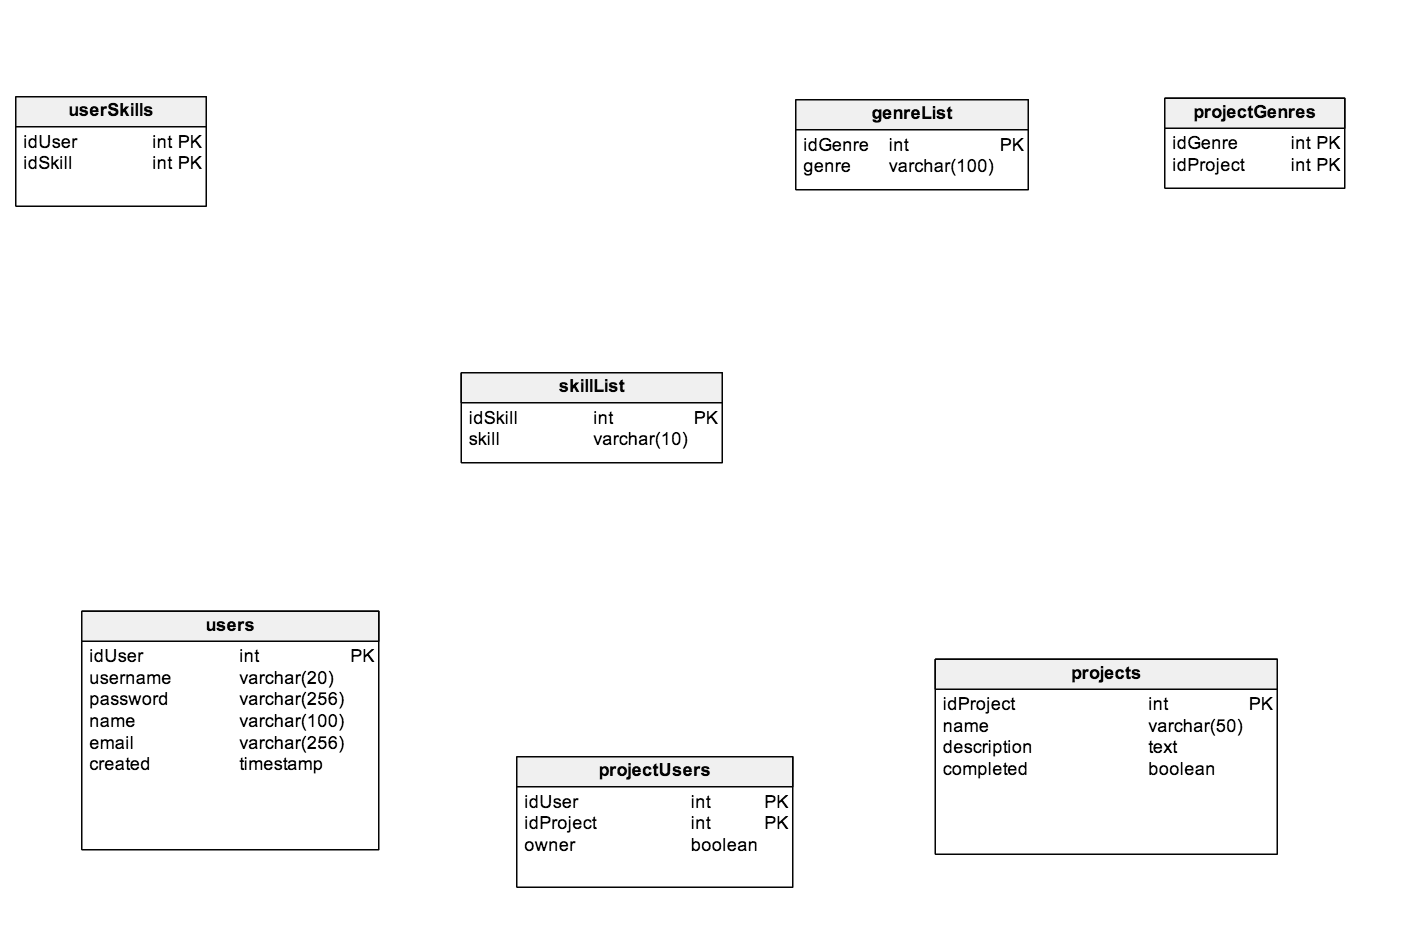
\includegraphics[width=180mm]{1.png}

As we continued implementing new features we quickly discovered that more and more tables were needed which made the database design even more complex. As we kept on adding more tables, it was important that we didn't duplicate data, which is why we made sure every table was in 3rd normal form. This meant that when updating, deleting or inserting rows we didn't have to make changes in multiple tables for the same data. This was mainly achieved by assessing which tables had a many-to-many relationship with each other and inserting a 'joining' table between them. \\
Backing up of the database has already been discussed, but to make things easier during testing and database migrating we kept a record of the table structure within sql files. This meant that tables could be created easily via the sql files, and adding test data could be done this way as well.
After some research, we also discovered that it was best to store uploaded files on the server file structure instead of inside of the database. This meant that links to the file path had to be stored in the database instead of the actual file. This allowed for sql queries to be much faster, as intending by the language. Adding large files into this database would have dramatically slowed down the queries, which would have been a big problem if the web app had been rolled out for commerical use.
\section{Acknowledgements}
\subsection{Libraries Used}
\begin{itemize}
\item blueimp file upload
This is used for a clean and attractive interface for users to upload multiple music, art and lyrics files easily and quickly, with no confusing elements. It's quick and colourful, meaning any user will find it easy and convenient to use
\item lightbox
This is an extremely attractive way to show photos on the page without having to design any specific page to hold them well. It Shows it as a modal over the current page if clicked, allowing users to quickly view photos in full glory
\item autosize text box
This is used to have input boxes grow as users enter data. This allows us a 'one size fits all' text box whenever necessary, so users can right as much or as little as they like, and the box will never look out of place
\item jPlayer + playlist
jPlayer was used as it is a free cross-browser media player, with a highly customiszble interface. It allowed us to make an audio player that was both simple and in-keeping with our websites style. The playlist addon allows us to present all files available for each section to the user and it links easily to the player.
\item jQuery + jQuery UI
Using jQuery allowed us to perform complex/cumbersome javascript scripts easily, without having advanced knowledge and in few lines. There is a choice of thousands of plugins which cover everything one needs in a website
\item jEditable + editInPlace 
jEditable is used on top of editInPlace to allow details of a project to be changed simply by clicking on them. This saves space, and means we don't have to spend time creating extra buttons or dialogs. It's quick and easy for users and allows one page to be both the display and editing page, giving a stream-lined experience
\end{itemize}

\subsection{Code/Pictures used?}
\subsection{Legal Issues}
The legal issues that would be involved in our app comprise of two different types:The issues surrounding the technologies and libraries we used and the issues surrounding the contents of the music/files shared on the site.
\subsubsection{Content}
This was the first issue we considered, when initialy planning the project. We realised that not only was there a problem with the sharing of one's own creation, but also the possibility of users sharing content they do not own and in doing so infringing on copyrighted material. We solved the first issue by having each be shared with a given licence from creativecommons.org, allowing users to pick one from the range available and limit how their work can be used however they want.

To solve the second issue, we would implement a flagging system so our more honest users could flag any suspected copyright infringment. Should we find any such materials we would have them deleted, and repeat offenders would be banned. Additionaly, we would have a disclaimer/copyright to show we own none of the material uploaded by users and that we reserve the right to remove any materials from the site, as well as advising users that it is illegal to upload such material.
\subsubsection{Technology}
The technologies we've used mean there hasn't been any legal problems with their use. jQuery, jQueryUI, jPlayer, jPlayerPlaylist, blueimp File Upload, LightBox and autosize are all open source, with the majority (all but LightBox and blueImp) being under the MIT licence.
\section{Conclusion}
\subsection{What We Have Done}
 \subsubsection{Navigation Bar}
 The navigation bar, as it suggests allows us to to navigate through our website. It has the function of allowing the user to search for people to follow, so that they can keep up to date with said persons work. Another feature is that you can search for projects, and people via genre, or skills. This means the user can find other users who have similar tastes, and also find projects which appeal to their skills or tastes. From the navigation bar the user can also create a project, the project requires names, skills and hte genre's it comes under.
\subsubsection{Home Page}
 The homepage is fully functional. It allows the user to login, and register to the website. On the homepage it gives brief details of what the website is about. When a user logs in or registers via the homepage it will redirect them to their profile page, so that they can start customising their profile. We have utilised javascript to add tasteful animation upon loading the webpage. When a user registers, his/her details are sent to the database so that they can hae their own profile, and are remembered upon return. Cookies were also implemented which saves the username. This allows the user to be automaitcally logged in when visiting the site. When logging out the cookie is removed.
 \subsubsection{Project Page}
 This page implements a list of players for each recorded section. Each section can have music uploaded to it, so that it can be voted on. The list is 'sortable' meaning that the user can arrange their sounds how they would like. Becaus we wanted to extend to all aspects of music production, album art and lyrics can be uploaded to the to the project page as well. From the project page the project leader has the ability to add personnel to their project, and also remove remove personnel. Group chat is also implemente
 \subsubsection{Profile Page}
 The profile page allows the user to upload images for their profile picture. Users can add skills they possess, so they can be easier identified for future project help. A description of the user can be added as well. Album portfolios can also be added to the page to showcase that particular talent.
\subsection{What We Have Not Done}
\subsubsection{Workflow}
 If a user wants to create a remix or alter existing sounds, we would like a system, similar in structureto git, so that a user can easily see how some of their sounds have evolved. This would ve very handy if a user would lke ot revert back to a previous sound, or just make sure the project is going in his/her desired direction. We felt that this system would be too complicated to implement in the given time period, and too much focus on this would compromise other area's fo the site.
\subsubsection{Tutorials/ Support Section}
 We did not have enough recources or knowledge to implement this, as it would require a vast knowledge base of various software and instrutments. The support section would have been implementable, but we felt we needed to get the core functionality working before we attempted this. A work around that we thought was allowing users to upload eir own tutorials, and of course increase their popularity. 
\subsubsection{Contests}
 Contests would of course would require a large user base to gain any credibility, but if we were to launch it. Users could vote for their favorite projects that have been realised. This would allow indie bands and Dj's to garner more fame, and therefore increase the sites popularity.
\subsection{What We Have Learned}
  \subsubsection{HTML and CSS}
  Some of the group had previously used HTML and CSS. Though others had not learnt any at all, so HTML and CSS was certainly more cumbersome for said members. Our group though came too grips with these languages, and we now feel competent using these languages. 
  \subsubsection{Jquery}
  Jquery was something all group members had to get used. It vastly increased our productivity giving us access to various plugins and functions. Using jquery made us realise how extensible a website could be, with sometime srelatively no effort. Using the plugins could be a pain though, as some had little documentation, making it fiddly.
  \subsubsection{PHP}
  Most of the group had contact with PHP, so that we could write values to the database. No members had previous eperience with PHP so there was certainly a learning curve. Though because it is well documented it was perhaps easier than alternatives like 'node.js'. 
  \subsubsection{PSQL}
  Mainly Ashley made use of the database, again he no previous experience and felt he came away with much more knowledge.
  \subsubsection{Group working}
  Working on web applictions was very different to other projects, because the work was very modular, allowing us to split the work well. Though because of our inexperience it was still sometimes easier to work together. Also it was very good fun generating the ideas for our webpages, and it taught us how to co-operate and build on ideas.
\subsection{What We Would Have Done Differently}
One major difference we would change is the use of git's branching ability and other advanced tools like tagging to keep track of points we were up to. This is because for the majority of the project we were using 1 branch for all of the design work, and occasionaly problems kept occuring when merging. Branching would have allowed us to develop sections individual and then merge the final product at certain points along the development timeline. \\
In addition, we found that 2 members of 
our group we working on the same page. Even though they were communicating about this and developing strategies on how to progress, it would have been better if they worked on different pages so no problems would have arised.\\
If we had more time, we would have liked to work on the design to make it look less 'boostrapy'. Although there is nothing wrong with the look, and bootstrap offers great components to base our website on, we really wanted a website with an individual look, which we didn't fully achieve.\\
Furthermore, we more time we would have liked to focus more on the functionality of the website. We spent a long time focussing little jQuery effects for validation, instead of developing other major features which would have added to web app overall.

\end{document}